\documentclass[12pt]{article}
\usepackage{amsfonts,amssymb}
\usepackage{amsmath}
\usepackage{amsthm}
\usepackage{hyperref}
\usepackage{graphicx}
\usepackage{listings}
%\documentstyle[12pt,amsfonts]{article}
%\documentstyle{article}

\setlength{\topmargin}{-.5in}
\setlength{\oddsidemargin}{0 in}
\setlength{\evensidemargin}{0 in}
\setlength{\textwidth}{6.5truein}
\setlength{\textheight}{8.5truein}
%
%\input ../adgeomcs/lamacb.tex
\input ../mac.tex
\input ../mathmac.tex
%
\input xy
\xyoption{all}
\def\fseq#1#2{(#1_{#2})_{#2\geq 1}}
\def\fsseq#1#2#3{(#1_{#3(#2)})_{#2\geq 1}}
\def\qleq{\sqsubseteq}
\newtheorem{theorem}{Theorem}
%cis51109hw1

%
\begin{document}
\begin{center}
\fbox{{\Large\bf Basic Probability}}\\
\vspace{1cm}
\end{center}


\medskip\noindent


\vspace{0.5cm}\noindent

\section*{What is an event}

An experiment is a procedure that results in one out of a number of possible outcomes. The set of all possible outcomes is called the sample space of the experiment. A subset of the sample space is called an event.

Examples are 

\begin{itemize}
\item Consider a simple example of an experiment in which a red and a blue die are thrown. We will denote a single outcome by an ordered pair where the first number denotes the outcome on the blue one and second number denotes the outcome on the red one.
Then the sample space is $S = \{(x,y)| 1 \le x \le 6, 1 \le y \le 6\}$.
Any subset of the sample space is called an event. So for instance the event $E$ or having doubles show up on the dice can be written explicitly as

$E = \{(1,1), (2,2), (3,3), (4,4), (5,5), (6,6)\}$.

\item Another common experiment is playing cards. Let us say we are playing poker and we get a 5 card hand. Obviously there are several possible outcomes. Every single outcome is one of the 5 element subsets of the set of 52 cards. 

The sample space therefore is of size ${52 \choose 5}$.

A particular event in this case for instance is a royal flush, which means A, K, Q, J and 10, all of the same suit. Let's call that event 

\begin{multline*}
R = \{\{A \clubsuit, K \clubsuit, Q \clubsuit, J \clubsuit, 10 \clubsuit\} , \{A \spadesuit, K \spadesuit, Q \spadesuit, J \spadesuit, 10 \spadesuit \}, \\
\{A \heartsuit, K \heartsuit, Q \heartsuit, J \heartsuit, 10 \heartsuit \} , \{ A \diamondsuit, K \diamondsuit, Q \diamondsuit, J \diamondsuit , 10 \diamondsuit \} \}
\end{multline*} 

There are 4 such royal flushes. 

\end{itemize}

\section*{Basic probability definition}
A natural question with regards to an experiment is to say, what is the likelihood (the probability) that a particular event occurs.

A probability distribution over an experiment with a sample space of $S$ is a function $p$ from $S$ to the set $[0,1]$.

Certain properties need to be satisfied by this probability distribution.

\begin{align*}
\sum_{s \in S} p(s) = 1
\end{align*}

The probability of the single outcome $s$ is $p(s)$. If $E \subseteq S$ is an event, then the probability of the event $E$ is  

\begin{align*}
p(E) = \sum_{s \in S} p(s) 
\end{align*}

This definition is especially useful when dealing with situations where not every outcome is equally likely. 

Loaded dice for instance. (More detail in the zybook)

Let's say a die is twice as likely to show up 4 as anything else. To make this work, we basically want to assign a value of 2/7 to $p(4)$ and a value of 1/7 to the probability of every other outcome.

Given these individual outcome probabilities, you can now work out the probabilities of any event

For example the event that the die shows a number greater than 3 becomes p(4) + p(5) + p (6) which is 4/7.

\section*{Uniform distribution}

In many scenarios, the probability of every outcome in the sample space is the same. The probability distribution in which every outcome has the same probability is called the uniform distribution. 

Since there are |S| outcomes and their probabilities sum to 1, under the uniform distribution, for each $s \in S$, $p(s) = 1/|S|$. The uniform distribution reduces questions about probabilities to questions about counting because for every event E,

\begin{align*}
p(E) = \frac{|E|}{|S|}
\end{align*}

\pagebreak

Example (from zybook - 11.1.1)

Consider a situation in which files are stored on a distributed network. Multiple copies of each files are stored around the network so that if one or more computers crash, the data is more likely to be available from at least one source. Suppose that three copies of a files are stored at different locations in a network of 30 computers and that at a particular moment, five random computers fail. Each subset of 5 computers are equally likely to be the five that have failed. What is the probability that there are no copies left of the file?

The experiment over here is choosing 5 computers that fail. So total number of distinct outcomes is ${30 \choose 5}$. Every computer is equally likely to fail. That means every subset of 5 is equally likely to fail. 

How many of these subsets have all 3 of the computers that contain this file? The file is in 3 of the computers, so we have to have all 3 of these computers being picked. But we still have a choice for the remaining 2 computers. 27 other computers exist. 2 of them have to be picked.

therefore $\frac{{27 \choose 2}}{{30 \choose 5}}$

\section*{Birthdays! - Complementary probability}

One of the cool applications of Probability is in the computation of how many people you need to have in a group before at least 2 of them have the same birthday.

Let's keep things simple and say that the year has 365 days (which works for most applications). 

Now obviously, if you have 366 people, the probability that at least 2 of them share the same birthday is 1. That sort of argument is what is generally referred to as the Pigeon hole principle (something that we do not cover much in this course).

Let's say you have m people. Now the number of ways in which those m people get birthdays assigned to them is - the first person has 365 choices, so does the second, so does the third and so on. So if we wrote out the sample space it would look like

$\{(b_1, b_2, \ldots, b_m)| 1 \le b_i \le 365 \}$.

We know how to count that. Product rule or the idea of Cartesian products. So the cardinality of this set is $365^m$.

How do we count the number of cases where at least 2 of these m people have the same birthday?
One way of doing it would be to say let's count the cases for exactly 2 having the same birthday then the cases for exactly 3 having the same birthday, and so on. But if $m$ is large, this is just going to be a huge pain!

Instead, we just look at what is called the complementary event and use this important idea

$P(A^c) = 1 - P(A)$ 

because after all, every outcome is either part of the event you want or not. And the probabilities have to total to 1.

So what is the complementary event in this case. The event that NONE of the $m$ people share a birthday. In how many ways can we have these $m$ people not share birthdays at all.

Think of it again as a sequencing/arrangement problem. Person 1 has 365 available to him/her as potential birthdays. Person 2 is not allowed to have a birthday on the same day, so that means 364 possible days. And now you get the idea...

That means the probability of the complement event = 

\begin{align*}
\frac{365 \times 364 \times \cdots (365-m+1)}{365^m}
\end{align*}

Therefore the probability of the event itself is

\begin{align*}
1 - \frac{365 \times 364 \times \cdots (365-m+1)}{365^m}
\end{align*}

This initially might seem like an uninteresting geeky expression until you start plugging numbers in. Here is a plot of number of people versus the probability of this event.

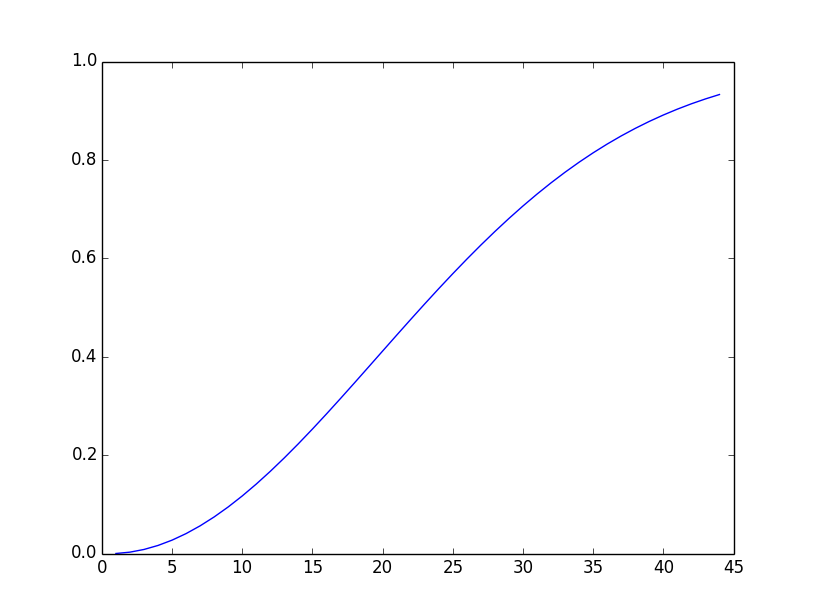
\includegraphics[scale=0.6]{birthday.png}

We have 42 in this class. There is a pretty good chance there is at least one pair that shares birthdays.

\section*{Application - Hashing and hashmaps}

Assume we have $n$ values and they are being hashed to 20 locations. Assume also that we do not have a hash function in mind yet, but just pick one completely at random. What is the probability that our hash function has no collisions!

If you think about this, it is actually the same thing as people and birthdays. Except the year now has 20 days instead of 365!!

So the probability that a randomly chosen hash function has no collisions is

\begin{align*}
\frac{P(20, n)}{20^n} = \frac{20 \cdot 19 \cdot 18 \cdots (20 - n + 1)} {20^n}
\end{align*}

Similar to the birthday problem it might be somewhat surprising to realize that the probability of some collision is actually fairly high.

\subsection*{Birthday attack!}

This part of the lecture is taken from a really nice set of slides that is linked to on the schedule page.

\href{http://www.facweb.iitkgp.ernet.in/~sourav/lecture_note9.pdf}{crytpo notes} has the complete version and since we are talking about this more as fun application of probability we will just refer to those slides.

\end{document}



